\documentclass[conference]{IEEEtran}
\IEEEoverridecommandlockouts

\usepackage{cite}
\usepackage{amsmath,amssymb,amsfonts}
\usepackage{graphicx}
\usepackage{textcomp}
\usepackage{xcolor}
\usepackage{booktabs}
\usepackage{multirow}
\usepackage{microtype}

\begin{document}

\title{MIS: Diagnosing Structural Bottlenecks in Copy-Paste Augmentation for Agricultural Object Detection}

\author{
    \IEEEauthorblockN{Huy Khanh Tran, Yuichiro Nomura, and Hiroshi Mineno}
    \IEEEauthorblockA{Graduate School of Integrated Science and Technology,
    Shizuoka University, Japan \\
    tran.huy.khanh.25@shizuoka.ac.jp}
}

\maketitle

\begin{abstract}
Copy-paste augmentation is widely used to increase training diversity, 
yet in dense agricultural scenes it often yields little or negative improvement for bounding-box detection.
We propose the Minimum Inference Score (MIS), a pre-augmentation diagnostic that scores object- and image-level difficulty by comparing a baseline detector's low-threshold predictions to existing ground truth.
On MinneApple and GWHD 2021, MIS aligns with size- and domain-level detection capacity without using domain labels.
Controlled copy-paste experiments show that failures are consistent with structural constraints---resolution ceilings for sub-resolution objects, density-limited distribution shift in already-crowded scenes, and domain-driven seed instability---rather than instance-selection heuristics.
By exposing these underlying bottlenecks, MIS provides a principled diagnostic tool, 
allowing practitioners to predict augmentation failure and avoid wasteful training cycles.

\end{abstract}

\begin{IEEEkeywords}
object detection, copy-paste augmentation, difficulty scoring, agricultural object detection, domain shift
\end{IEEEkeywords}
% ----------------------------------------------------------

\section{Introduction}
Copy-paste augmentation \cite{kisantal2019augmentation, ghiasi2021simple} composits cropped labeled instances into training images to increase effective sampling.
Kisantal et al.\ \cite{kisantal2019augmentation} reported gains for small objects on sparse COCO settings, with trade-offs across scales, and Ghiasi et al.\ \cite{ghiasi2021simple} showed strong results for instance segmentation.
However, bounding-box detection in agricultural imagery operates under harsher constraints: high object density, frequent sub-resolution instances, occlusion, and multi-domain acquisition.
In practice, copy-paste in this regime often produces inconsistent or negative gains, forcing expensive multi-seed trial-and-error.

We introduce the \textbf{Minimum Inference Score (MIS)}, a lightweight pre-augmentation diagnostic computed from a trained baseline detector.
MIS does not aim to improve AP directly; it estimates whether copy-paste is structurally plausible \textit{before} augmentation.
On MinneApple \cite{hani2020minneapple} and GWHD 2021 \cite{david2021global},
 results indicate that copy-paste failures are dominated by 
 dataset bottlenecks (resolution, density-limited shift, and domain instability) 
 rather than selection strategy.


\section{Methodology}
\subsection{Scoring Formulation}
Let $G(I)$ denote ground-truth boxes in image $I$. A trained baseline detector
produces predictions $p$ with confidence $c_p$ at a low threshold
$\tau_{\mathrm{conf}}{=}0.001$ (to retain near-miss candidates rather than enforce a deployment threshold).
For each ground-truth object $g\in G(I)$, define the set of overlapping predictions
\[
\mathcal{P}(g) = \{p : \mathrm{IoU}(p,g) \ge \tau_{\mathrm{IoU}}\}, \;\;\; \tau_{\mathrm{IoU}}{=}0.5,
\]
allowing multiple candidates per $g$.
With $u_p=\mathrm{IoU}(p,g)$, the \textit{Object Difficulty Score} is
\begin{equation}
S_{\mathrm{obj}}(g) =
\begin{cases}
  \min_{p \in \mathcal{P}(g)}
    \left[\alpha(1{-}c_p) + \beta(1{-}u_p)\right],
    & \mathcal{P}(g) \neq \varnothing \\[3pt]
  \alpha + \beta, & \mathcal{P}(g) = \varnothing
\end{cases}
\label{eq:obj}
\end{equation}
with $\alpha{=}\beta{=}0.5$. The minimum selects the detector's best-aligned attempt for $g$;
unmatched objects receive the maximum score.

The \textit{Image Difficulty Score} combines mean object difficulty with a false-positive term:
\begin{equation}
S_{\mathrm{img}}(I)
  = \frac{1}{|G(I)|}\sum_{g \in G(I)} S_{\mathrm{obj}}(g)
  + w_2 \cdot \mathrm{FPrate}(I),
\label{eq:img}
\end{equation}
where $\mathrm{FPrate}(I)$ is the number of unmatched predictions per image (computed at the same
$\tau_{\mathrm{conf}}$ and $\tau_{\mathrm{IoU}}$). We set $w_2$ by grid search to balance the contribution
of misses and false positives by equalizing Pearson correlations
$r(S_{\mathrm{img}},\mathrm{miss\,rate})$ and $r(S_{\mathrm{img}},\mathrm{FP\,rate})$ on the training set.

% \subsection{Augmentation Protocol}
% We train a YOLOv8s baseline detector and compute $S_{\mathrm{img}}$ for all training images.
% Images are ranked and partitioned into equal tertiles. We evaluate four copy-paste conditions:
% \textbf{Random}, \textbf{Score High}, \textbf{Score Medium}, and \textbf{Score Low}. In each MIS-guided condition,
% both (i) the destination image pool and (ii) the source object pool are drawn from the same tertile.

% Inspired by the work of Kisantal et al.\ \cite{kisantal2019augmentation}, 
% we expand training data by 30\% using unblended same-image copy-paste: 2--8 pasted objects per image, scale $[0.9,1.1]$, rotation $\pm15^\circ$,
% and maximum reuse of $3{\times}$ per image and per object. All other training settings follow the default
% YOLOv8 protocol unless stated.

\subsection{Augmentation Protocol}
We train a YOLOv8s baseline detector and compute $S_{\mathrm{img}}$ and $S_{\mathrm{obj}}$ for all training images, objects.
Images (by $S_{\mathrm{img}}$) and objects (by $S_{\mathrm{obj}}$) are ranked and partitioned into equal tertiles.
We evaluate four copy-paste conditions: \textbf{Random}, \textbf{Score High}, \textbf{Score Medium}, and \textbf{Score Low}.
In each MIS-guided condition, destination images are sampled from the corresponding image tertile, and pasted objects are sampled from the corresponding object tertile \emph{within the same image}.
Inspired by Kisantal et al.\ \cite{kisantal2019augmentation}, we expand training data by 30\% using unblended within-image copy-paste:
2--8 pasted objects per image, scale $[0.9,1.1]$, rotation $\pm15^\circ$, and maximum reuse of $3{\times}$ per image and per object.
All other training settings follow the default YOLOv8 protocol unless stated.


\section{Results: Validation, Failure Modes, and Diagnostic Use}
\subsection{MIS validation}
\textbf{MinneApple (size-level).}
$S_{\mathrm{obj}}$ is inversely associated with detection capacity across size groups (Spearman $r_s{=}{-}0.82$):
the top-difficulty tertile is dominated by \textit{Very Small} instances ($\le400$\,px$^2$), where baseline AP is near-zero (AP$=0.071$).
This indicates a resolution-driven information bottleneck: increasing frequency of these instances via copy-paste is unlikely to produce a stable learning signal.

\textbf{GWHD 2021 (domain-level).}
Without using domain labels, MIS ranks images such that per-domain median difficulty strongly anticorrelates with domain AP
(Pearson $r{=}{-}0.9047$, Spearman $r_s{=}{-}0.8989$; Fig.~\ref{fig:gwhd_domain}),
supporting MIS as a proxy for domain difficulty derived from baseline detector behavior.

\begin{table}[t]
\centering
\caption{MIS validation on MinneApple: size-level difficulty aligns with AP.}
\label{tab:size_validation}
\footnotesize
\setlength{\tabcolsep}{3.5pt}
\renewcommand{\arraystretch}{0.95}
\begin{tabular}{lccc}
\toprule
\textbf{Category} & \textbf{AP} & \textbf{Mean $S_{\mathrm{obj}}$} & \textbf{Top tertile} \\
\midrule
Very Small ($\le$400\,px$^2$) & 0.071 & 0.152 & 64.4\% \\
Small (400--1024\,px$^2$)     & 0.270 & 0.076 & 33.9\% \\
Medium ($>$1024\,px$^2$)      & 0.493 & 0.053 & 1.7\% \\
\bottomrule
\end{tabular}
\end{table}

\begin{figure}[t]
  \centering
  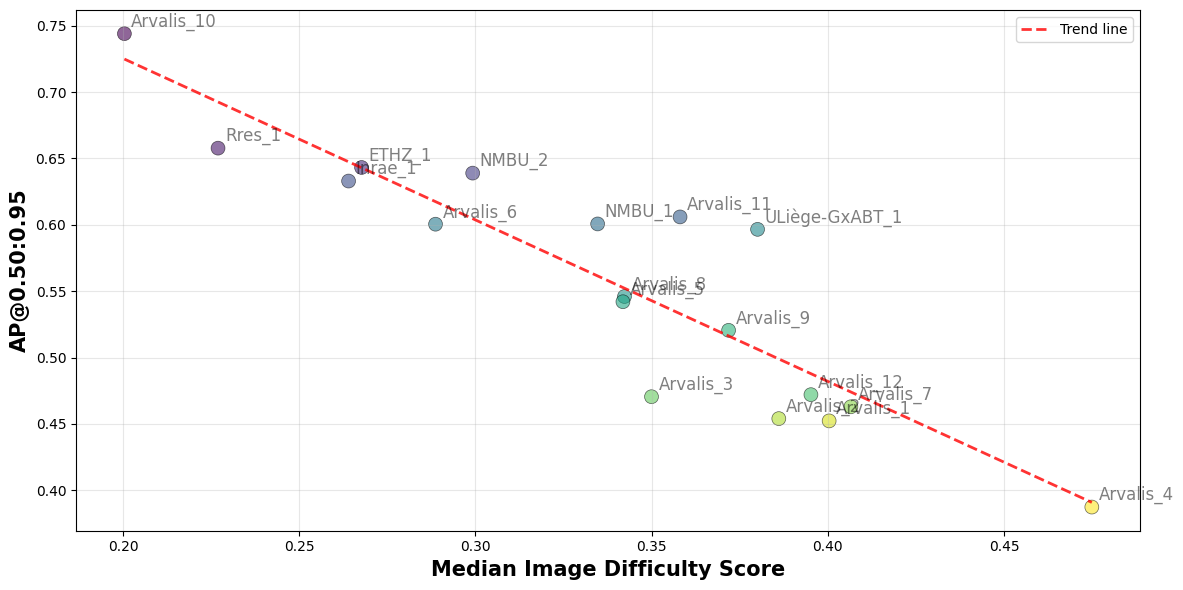
\includegraphics[width=\columnwidth]{gwhd_domain_score.png}
  \caption{GWHD 2021: per-domain AP vs median image difficulty (MIS).}
  \label{fig:gwhd_domain}
\end{figure}

\subsection{Copy-paste outcomes and failure analysis}
\textbf{MinneApple: insufficient distribution shift under dense, sub-resolution conditions.}
Across all four copy-paste conditions, AP changes are negligible and negative within seed variance (Table~\ref{tab:aug}).
The critical control is \textbf{Score Low}: it produces the largest shift in the training size mix toward the test distribution (higher Medium fraction),
yet yields no AP improvement.
This weakens ``suboptimal instance selection'' as the primary explanation and is more consistent with structural constraints:
(i) a resolution ceiling dominated by Very Small objects (Table~\ref{tab:size_validation}),
and (ii) a marginal density increase that is small relative to the already-dense baseline (Obj/Img changes by ${\sim}1$--$2$),
limiting the ability of copy-paste to introduce meaningfully new training signal.

\textbf{GWHD 2021: domain-linked seed instability.}
Score High augmentation yields near-zero mean gain but 
large seed sensitivity: across three seeds, performance ranges from a gain of 
$+0.042$ AP (seed 456)
to a drop of $-0.055$ AP (seed 123).
Given the strong domain difficulty--AP anticorrelation (Fig.~\ref{fig:gwhd_domain}), this variance is consistent with high-difficulty images concentrating in minority domains;
score-guided sampling can therefore amplify domain imbalance, making outcomes sensitive to sampling order and initialization.
Practically, this can produce misleading ``lucky-seed'' improvements.

\begin{table}[t]
\centering
\caption{MinneApple copy-paste results (3-seed mean). No condition yields a reliable gain.}
\label{tab:aug}
\footnotesize
\setlength{\tabcolsep}{3.0pt}
\renewcommand{\arraystretch}{0.95}
\begin{tabular}{lccccc}
\toprule
\textbf{Condition} & \textbf{Obj/Img} & \textbf{V.\,Small} & \textbf{Small} & \textbf{Medium} & \textbf{AP$\pm\sigma$} \\
\midrule
Test set      & 37.11 & 17.2\% & 38.1\% & 44.7\% & --- \\
\midrule
Baseline      & 42.6  & 23.1\% & 50.5\% & 26.4\% & $0.353\pm0.005$ \\
Random CP     & 44.0  & 23.5\% & 49.9\% & 26.5\% & $0.346\pm0.005$ \\
Score High    & 43.9  & 26.5\% & 49.5\% & 23.9\% & $0.350\pm0.007$ \\
Score Medium  & 43.2  & 22.6\% & 50.8\% & 26.6\% & $0.348\pm0.006$ \\
Score Low     & 42.4  & 20.0\% & 48.5\% & 31.5\% & $0.348\pm0.003$ \\
\bottomrule
\end{tabular}
\end{table}

\subsection{Pre-augmentation diagnostic checklist}
Across these two benchmarks, MIS supports a practical triage computed from baseline outputs:
\textbf{(1) Information bottleneck:} if high MIS objects concentrate in regimes with near-zero baseline AP (e.g., sub-resolution sizes),
copy-paste is unlikely to help because the detector lacks usable capacity in that regime.
\textbf{(2) Density-limited shift:} if baseline object density is already high, the achievable proportional density increase at the chosen augmentation ratio is small,
limiting distribution shift even with ``correct'' sampling.
\textbf{(3) Domain instability:} if high MIS images cluster in minority domains (observable via domain-level difficulty--AP anticorrelation),
score-guided augmentation may amplify domain imbalance and increase seed variance.

% ----------------------------------------------------------
\section{Conclusion}
MIS reframes copy-paste augmentation from trial-and-error into a pre-augmentation diagnostic.
On MinneApple and GWHD 2021, MIS aligns with size- and domain-level detection capacity and highlights failure modes that are consistent with dense, sub-resolution scenes
and domain-driven instability.
These findings are retrospective on two benchmarks under a fixed copy-paste protocol; prospective validation on datasets where copy-paste yields consistent gains remains necessary.

When MIS indicates a resolution ceiling (near-zero AP in the dominant hard regime), simply duplicating pixels via copy-paste is unlikely to be sufficient.
A plausible next direction is to evaluate augmentations that \emph{increase effective information content} for hard cases (e.g., controlled super-resolution,
domain-conditioned synthesis, or inpainting-based instance generation), while explicitly validating that generated samples remain in-distribution.

\begin{thebibliography}{00}

\bibitem{kisantal2019augmentation}
M.~Kisantal, Z.~Wojna, J.~Murawski, J.~Naruniec, and K.~Kyriakopoulos,
``Augmentation for small object detection,''
in \textit{Proc. Int. Conf. Adv. Comput., Commun. Informat.\ (ICACCI)}, 2019, pp.~193--197.

\bibitem{ghiasi2021simple}
G.~Ghiasi \textit{et~al.},
``Simple copy-paste is a strong data augmentation method for instance segmentation,''
in \textit{Proc. IEEE/CVF CVPR}, 2021, pp.~2918--2928.

\bibitem{hani2020minneapple}
N.~Hani, P.~Roy, and B.~Bhanu,
``MinneApple: A benchmark dataset for apple detection and segmentation,''
\textit{IEEE Robot.\ Autom.\ Lett.}, vol.~5, no.~2, pp.~852--858, 2020.

\bibitem{david2021global}
E.~David \textit{et~al.},
``Global Wheat Head Detection (GWHD) dataset,''
\textit{Plant Phenomics}, 2021.

\end{thebibliography}

\end{document}

% \documentclass[conference]{IEEEtran}
% \IEEEoverridecommandlockouts

% \usepackage{cite}
% \usepackage{amsmath,amssymb,amsfonts}
% \usepackage{graphicx}
% \usepackage{textcomp}
% \usepackage{xcolor}
% \usepackage{booktabs}
% \usepackage{multirow}
% \usepackage{microtype}

% \begin{document}

% \title{MIS: Diagnosing Structural Bottlenecks in Copy-Paste Augmentation for Agricultural Object Detection}

% \author{
%     \IEEEauthorblockN{Huy Khanh Tran, Yuichiro Nomura, and Hiroshi Mineno}
%     \IEEEauthorblockA{Graduate School of Integrated Science and Technology,
%     Shizuoka University, Japan \\
%     tran.huy.khanh.25@shizuoka.ac.jp}
% }

% \maketitle

% \begin{abstract}
% Copy-paste augmentation is widely used to increase training diversity, yet in dense agricultural scenes it often yields little or negative improvement for bounding-box detection.
% We propose the Minimum Inference Score (MIS), a pre-augmentation diagnostic that scores object- and image-level difficulty by comparing a baseline detector's low-threshold predictions to existing ground truth.
% On MinneApple and GWHD 2021, MIS aligns with size- and domain-level detection capacity without using domain labels.
% Controlled copy-paste experiments show that failures are consistent with structural constraints---resolution ceilings for sub-resolution objects, density-limited distribution shift in already-crowded scenes, and domain-driven seed instability---rather than instance-selection heuristics.
% MIS enables practitioners to screen for these conditions before running costly augmentation trials.
% \end{abstract}

% \begin{IEEEkeywords}
% object detection, copy-paste augmentation, difficulty scoring, agricultural detection, domain shift
% \end{IEEEkeywords}

% % ----------------------------------------------------------
% \section{Introduction}
% Copy-paste augmentation \cite{kisantal2019augmentation, ghiasi2021simple} composits cropped labeled instances into training images to increase effective sampling.
% Kisantal et al.\ \cite{kisantal2019augmentation} reported gains for small objects on sparse COCO settings, with trade-offs across scales, and Ghiasi et al.\ \cite{ghiasi2021simple} showed strong results for instance segmentation.
% However, bounding-box detection in agricultural imagery operates under harsher constraints: high object density, frequent sub-resolution instances, occlusion, and multi-domain acquisition.
% In practice, copy-paste in this regime often produces inconsistent or negative gains, forcing expensive multi-seed trial-and-error.

% We introduce the \textbf{Minimum Inference Score (MIS)}, a lightweight pre-augmentation diagnostic computed from a trained baseline detector.
% MIS does not aim to improve AP directly; it estimates whether copy-paste is structurally plausible \textit{before} augmentation.
% On MinneApple \cite{hani2020minneapple} and GWHD 2021 \cite{david2021global}, results indicate that copy-paste failures are dominated by dataset bottlenecks (resolution, density-limited shift, and domain instability) rather than selection strategy.

% % ----------------------------------------------------------
% \section{Methodology}
% \subsection{Scoring Formulation}
% Let $G(I)$ denote ground-truth boxes in image $I$.
% A trained baseline detector produces predictions $p$ with confidence $c_p$ at a low threshold
% $\tau_{\mathrm{conf}}{=}0.001$ to retain near-miss candidates.
% For each ground-truth object $g\in G(I)$, define the set of overlapping predictions
% \[
% \mathcal{P}(g) = \{p : \mathrm{IoU}(p,g) \ge \tau_{\mathrm{IoU}}\}, \;\;\; \tau_{\mathrm{IoU}}{=}0.5,
% \]
% allowing multiple candidates per $g$.
% With $u_p=\mathrm{IoU}(p,g)$, the \textit{Object Difficulty Score} is
% \begin{equation}
% S_{\mathrm{obj}}(g) =
% \begin{cases}
%   \min_{p \in \mathcal{P}(g)}
%     \left[\alpha(1{-}c_p) + \beta(1{-}u_p)\right],
%     & \mathcal{P}(g) \neq \varnothing \\[3pt]
%   \alpha + \beta, & \mathcal{P}(g) = \varnothing
% \end{cases}
% \label{eq:obj}
% \end{equation}
% with $\alpha{=}\beta{=}0.5$.
% The minimum selects the detector's best-aligned attempt for $g$; unmatched objects receive the maximum score.

% The \textit{Image Difficulty Score} combines mean object difficulty with a false-positive term:
% \begin{equation}
% S_{\mathrm{img}}(I)
%   = \frac{1}{|G(I)|}\sum_{g \in G(I)} S_{\mathrm{obj}}(g)
%   + w_2 \cdot \mathrm{FPrate}(I),
% \label{eq:img}
% \end{equation}
% where $\mathrm{FPrate}(I)$ is the number of unmatched predictions per image (computed at the same
% $\tau_{\mathrm{conf}}$ and $\tau_{\mathrm{IoU}}$).
% We choose $w_2$ by grid search to balance miss and false-positive contributions by matching Pearson correlations
% $r(S_{\mathrm{img}},\mathrm{miss\,rate})$ and $r(S_{\mathrm{img}},\mathrm{FP\,rate})$ on the training set.

% \subsection{Augmentation Protocol}
% We train a YOLOv8s baseline detector and compute $S_{\mathrm{img}}$ for all training images.
% Images are ranked and partitioned into equal tertiles.
% We evaluate four copy-paste conditions: \textbf{Random}, \textbf{Score High}, \textbf{Score Medium}, and \textbf{Score Low}.
% In each MIS-guided condition, destination images and source objects are drawn from the same tertile.
% We expand training data by 30\% using unblended same-image copy-paste \cite{kisantal2019augmentation}:
% 2--8 objects/image, scale $[0.9,1.1]$, rotation $\pm15^\circ$,
% and maximum reuse of $3{\times}$ per image and per object.
% All other training settings follow the default YOLOv8 protocol unless stated.

% % ----------------------------------------------------------
% \section{Results: Validation, Failure Modes, and Diagnostic Use}
% \subsection{MIS validation}
% \textbf{MinneApple (size-level).}
% $S_{\mathrm{obj}}$ is inversely associated with detection capacity across size groups (Spearman $r_s{=}{-}0.82$):
% the top-difficulty tertile is dominated by \textit{Very Small} instances ($\le400$\,px$^2$), where baseline AP is near-zero (AP$=0.071$).
% This indicates a resolution-driven bottleneck: duplicating sub-resolution instances via copy-paste is unlikely to yield a stable learning signal.

% \textbf{GWHD 2021 (domain-level).}
% Without using domain labels, MIS ranks images such that per-domain median difficulty strongly anticorrelates with domain AP
% (Pearson $r{=}{-}0.9047$, Spearman $r_s{=}{-}0.8989$; Fig.~\ref{fig:gwhd_domain}),
% supporting MIS as a proxy for domain difficulty derived from baseline detector behavior.

% \begin{table}[t]
% \centering
% \caption{MIS validation on MinneApple: size-level difficulty aligns with AP.}
% \label{tab:size_validation}
% \footnotesize
% \setlength{\tabcolsep}{3.5pt}
% \renewcommand{\arraystretch}{0.95}
% \begin{tabular}{lccc}
% \toprule
% \textbf{Category} & \textbf{AP} & \textbf{Mean $S_{\mathrm{obj}}$} & \textbf{Top tertile} \\
% \midrule
% Very Small ($\le$400\,px$^2$) & 0.071 & 0.152 & 64.4\% \\
% Small (400--1024\,px$^2$)     & 0.270 & 0.076 & 33.9\% \\
% Medium ($>$1024\,px$^2$)      & 0.493 & 0.053 & 1.7\% \\
% \bottomrule
% \end{tabular}
% \end{table}

% \begin{figure}[t]
%   \centering
%   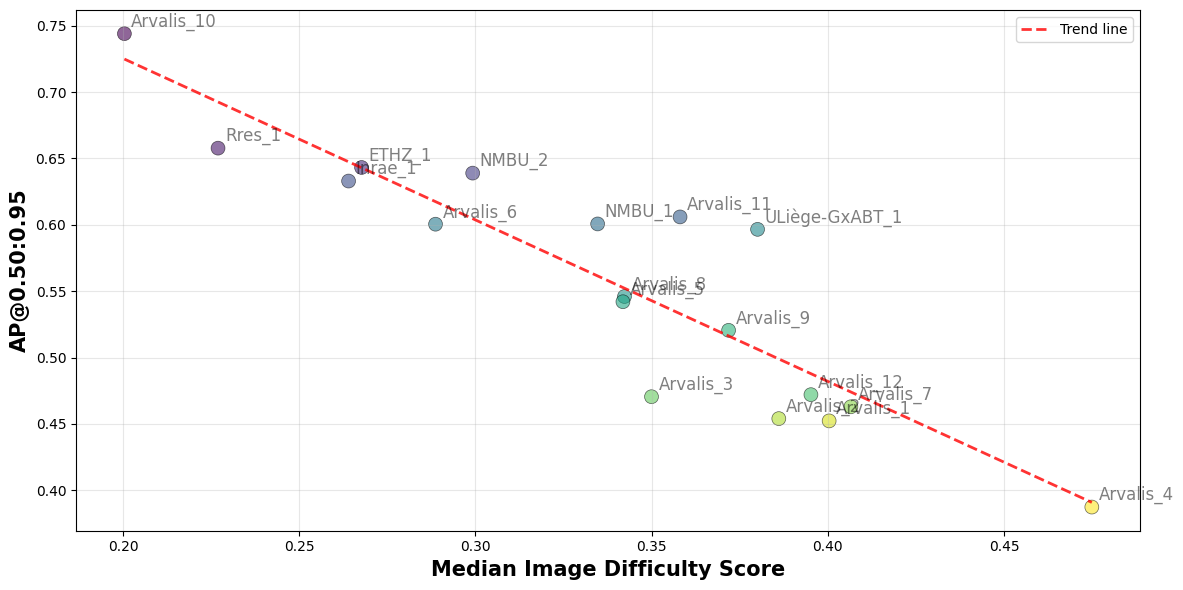
\includegraphics[width=\columnwidth]{gwhd_domain_score.png}
%   \caption{GWHD 2021: per-domain AP vs median image difficulty (MIS).}
%   \label{fig:gwhd_domain}
% \end{figure}

% \subsection{Copy-paste outcomes and failure analysis}
% \textbf{MinneApple: insufficient distribution shift under dense, sub-resolution conditions.}
% Across all four copy-paste conditions, AP changes are negligible and negative within seed variance (Table~\ref{tab:aug}).
% The critical control is \textbf{Score Low}: it increases the Medium fraction (31.5\%) relative to baseline (26.4\%),
% yet yields no AP improvement.
% This weakens ``suboptimal instance selection'' as the primary explanation and is more consistent with structural constraints:
% (i) a resolution ceiling dominated by Very Small objects (Table~\ref{tab:size_validation}),
% and (ii) a marginal density increase relative to the already-dense baseline (Obj/Img changes by ${\sim}1$--$2$),
% limiting the ability of copy-paste to introduce meaningfully new training signal.

% \textbf{GWHD 2021: domain-linked seed instability.}
% Score High augmentation yields near-zero mean gain but large seed sensitivity: across three seeds,
% performance ranges from a gain of $+0.042$ AP (seed 456) to a drop of $-0.055$ AP (seed 123).
% Given the strong domain difficulty--AP anticorrelation (Fig.~\ref{fig:gwhd_domain}), this variance is consistent with hard images concentrating in minority domains;
% score-guided sampling can therefore amplify domain imbalance, making outcomes sensitive to sampling order and initialization.

% \begin{table}[t]
% \centering
% \caption{MinneApple copy-paste results (3-seed mean). No condition yields a reliable gain.}
% \label{tab:aug}
% \footnotesize
% \setlength{\tabcolsep}{3.0pt}
% \renewcommand{\arraystretch}{0.95}
% \begin{tabular}{lccccc}
% \toprule
% \textbf{Condition} & \textbf{Obj/Img} & \textbf{V.\,Small} & \textbf{Small} & \textbf{Medium} & \textbf{AP$\pm\sigma$} \\
% \midrule
% Baseline      & 42.6  & 23.1\% & 50.5\% & 26.4\% & $0.353\pm0.005$ \\
% Random CP     & 44.0  & 23.5\% & 49.9\% & 26.5\% & $0.346\pm0.005$ \\
% Score High    & 43.9  & 26.5\% & 49.5\% & 23.9\% & $0.350\pm0.007$ \\
% Score Medium  & 43.2  & 22.6\% & 50.8\% & 26.6\% & $0.348\pm0.006$ \\
% Score Low     & 42.4  & 20.0\% & 48.5\% & 31.5\% & $0.348\pm0.003$ \\
% \bottomrule
% \end{tabular}
% \end{table}

% \subsection{Pre-augmentation diagnostic checklist}
% Across these benchmarks, MIS supports a practical triage from baseline outputs:
% (i) \textit{Information bottleneck}---hard objects concentrate in regimes with near-zero AP (e.g., sub-resolution sizes), implying limited usable capacity;
% (ii) \textit{Density-limited shift}---high baseline density implies that typical copy-paste ratios induce only marginal distribution shift even with ``correct'' sampling;
% (iii) \textit{Domain instability}---hard images cluster in minority domains (Fig.~\ref{fig:gwhd_domain}), so score-guided sampling can amplify imbalance and increase seed variance.

% % ----------------------------------------------------------
% \section{Conclusion}
% MIS reframes copy-paste augmentation from trial-and-error into a pre-augmentation diagnostic.
% On MinneApple and GWHD 2021, MIS aligns with size- and domain-level detection capacity and highlights failure modes consistent with dense, sub-resolution scenes and domain-driven instability.
% These findings are retrospective on two benchmarks under a fixed copy-paste protocol; prospective validation on datasets where copy-paste yields consistent gains remains necessary.
% When MIS indicates a resolution ceiling (near-zero AP in the dominant hard regime), duplicating pixels via copy-paste is unlikely to be sufficient.
% A plausible next direction is to evaluate augmentations that increase effective information content for hard cases (e.g., controlled super-resolution, domain-conditioned synthesis, or inpainting-based instance generation), while validating that generated samples remain in-distribution.

% {\footnotesize
% \begin{thebibliography}{00}
% \bibitem{kisantal2019augmentation}
% M.~Kisantal, Z.~Wojna, J.~Murawski, J.~Naruniec, and K.~Kyriakopoulos,
% ``Augmentation for small object detection,''
% in \textit{Proc. Int. Conf. Adv. Comput., Commun. Informat.\ (ICACCI)}, 2019, pp.~193--197.

% \bibitem{ghiasi2021simple}
% G.~Ghiasi \textit{et~al.},
% ``Simple copy-paste is a strong data augmentation method for instance segmentation,''
% in \textit{Proc. IEEE/CVF CVPR}, 2021, pp.~2918--2928.

% \bibitem{hani2020minneapple}
% N.~Hani, P.~Roy, and B.~Bhanu,
% ``MinneApple: A benchmark dataset for apple detection and segmentation,''
% \textit{IEEE Robot.\ Autom.\ Lett.}, vol.~5, no.~2, pp.~852--858, 2020.

% \bibitem{david2021global}
% E.~David \textit{et~al.},
% ``Global Wheat Head Detection (GWHD) dataset,''
% \textit{Plant Phenomics}, 2021.
% \end{thebibliography}
% }

% \end{document}

% \documentclass[conference]{IEEEtran}
% \IEEEoverridecommandlockouts

% \usepackage{cite}
% \usepackage{amsmath,amssymb,amsfonts}
% \usepackage{graphicx}
% \usepackage{textcomp}
% \usepackage{xcolor}
% \usepackage{booktabs}
% \usepackage{multirow}
% \usepackage{microtype}

% \begin{document}

% \title{MIS: Diagnosing Structural Bottlenecks in Copy-Paste Augmentation for Agricultural Object Detection}

% \author{
%     \IEEEauthorblockN{Huy Khanh Tran, Yuichiro Nomura, and Hiroshi Mineno}
%     \IEEEauthorblockA{Graduate School of Integrated Science and Technology,
%     Shizuoka University, Japan \\
%     tran.huy.khanh.25@shizuoka.ac.jp}
% }

% \maketitle

% \begin{abstract}
% Copy-paste augmentation is widely used to increase training diversity, yet in dense agricultural scenes it often yields little or negative improvement for bounding-box detection.
% We propose the Minimum Inference Score (MIS), a pre-augmentation diagnostic that scores object- and image-level difficulty by comparing a baseline detector's low-threshold predictions to existing ground truth.
% On MinneApple and GWHD 2021, MIS aligns with sizeand domain-level detection capacity without using domain labels.
% Controlled copy-paste experiments show that failures are consistent with structural constraints---resolution ceilings for sub-resolution objects, density-limited distribution shift in already-crowded scenes, and domain-driven seed instability---rather than instance-selection heuristics.
% MIS enables practitioners to screen for these conditions before running costly augmentation trials.
% \end{abstract}

% \begin{IEEEkeywords}
% object detection, copy-paste augmentation, difficulty scoring, agricultural detection, domain shift
% \end{IEEEkeywords}

% % ----------------------------------------------------------
% \section{Introduction}
% Copy-paste augmentation \cite{kisantal2019augmentation, ghiasi2021simple} composites cropped labeled instances into training images to increase effective sampling.
% Kisantal et al.\ \cite{kisantal2019augmentation} reported gains for small objects on sparse COCO settings, with trade-offs across scales, and Ghiasi et al.\ \cite{ghiasi2021simple} showed strong results for instance segmentation.
% However, bounding-box detection in agricultural imagery operates under harsher constraints: high object density, frequent sub-resolution instances, occlusion, and multi-domain acquisition.
% In practice, copy-paste in this regime often produces inconsistent or negative gains, forcing expensive multi-seed trial-and-error.

% We introduce the \textbf{Minimum Inference Score (MIS)}, a lightweight pre-augmentation diagnostic computed from a trained baseline detector.
% MIS does not aim to improve AP directly; it estimates whether copy-paste is structurally plausible \textit{before} augmentation.
% On MinneApple \cite{hani2020minneapple} and GWHD 2021 \cite{david2021global}, results indicate that copy-paste failures are dominated by dataset bottlenecks (resolution, density-limited shift, and domain instability) rather than selection strategy.

% % ----------------------------------------------------------
% \section{Methodology}
% \subsection{Scoring Formulation}
% Let $G(I)$ denote ground-truth boxes in image $I$.
% A trained baseline detector produces predictions $p$ with confidence $c_p$ at a low threshold
% $\tau_{\mathrm{conf}}{=}0.001$ to retain near-miss candidates.
% For each ground-truth object $g\in G(I)$, define the set of overlapping predictions
% \[
% \mathcal{P}(g) = \{p : \mathrm{IoU}(p,g) \ge \tau_{\mathrm{IoU}}\}, \;\;\; \tau_{\mathrm{IoU}}{=}0.5,
% \]
% allowing multiple candidates per $g$.
% With $u_p=\mathrm{IoU}(p,g)$, the \textit{Object Difficulty Score} is
% \begin{equation}
% S_{\mathrm{obj}}(g) =
% \begin{cases}
%   \min_{p \in \mathcal{P}(g)}
%     \left[\alpha(1{-}c_p) + \beta(1{-}u_p)\right],
%     & \mathcal{P}(g) \neq \varnothing \\[3pt]
%   \alpha + \beta, & \mathcal{P}(g) = \varnothing
% \end{cases}
% \label{eq:obj}
% \end{equation}
% with $\alpha{=}\beta{=}0.5$.
% The minimum selects the detector's best-aligned attempt for $g$; unmatched objects receive the maximum score.

% The \textit{Image Difficulty Score} combines mean object difficulty with a false-positive term:
% \begin{equation}
% S_{\mathrm{img}}(I)
%   = \frac{1}{|G(I)|}\sum_{g \in G(I)} S_{\mathrm{obj}}(g)
%   + w_2 \cdot \mathrm{FPrate}(I),
% \label{eq:img}
% \end{equation}
% where $\mathrm{FPrate}(I)$ counts predictions in image $I$ with $c_p \ge \tau_{\mathrm{conf}}$
% that fail to match any $g\in G(I)$ at $\tau_{\mathrm{IoU}}$
% (i.e., $\max_{g\in G(I)} \mathrm{IoU}(p,g) < \tau_{\mathrm{IoU}}$).
% We choose $w_2$ by grid search to balance miss and false-positive contributions by matching Pearson correlations
% $r(S_{\mathrm{img}},\mathrm{miss\,rate})$ and $r(S_{\mathrm{img}},\mathrm{FP\,rate})$ on the training set.

% \subsection{Augmentation Protocol}
% We train a YOLOv8s baseline detector and compute $S_{\mathrm{img}}$ for all training images and $S_{\mathrm{obj}}$ for all labeled objects.
% Training images are ranked by $S_{\mathrm{img}}$ and partitioned into equal tertiles; objects are ranked by $S_{\mathrm{obj}}$ and partitioned analogously.
% We evaluate four conditions: \textbf{Random}, \textbf{Score High}, \textbf{Score Medium}, and \textbf{Score Low}.
% In each MIS-guided condition, destination objects and images are sampled from the 
% corresponding $S_{\mathrm{img}}$ tertile.
% We expand training data by 30\% using unblended within-image copy-paste \cite{kisantal2019augmentation}:
% 2--8 objects/image, scale $[0.9,1.1]$, rotation $\pm15^\circ$,
% and maximum reuse of $3{\times}$ per image and per object.
% All other training settings follow the default YOLOv8 protocol unless stated, 
% and all conditions use the same detector, image size, and evaluation settings.


% % ----------------------------------------------------------
% \section{Results: Validation, Failure Modes, and Diagnostic Use}
% \subsection{MIS validation}
% \textbf{MinneApple (size-level).}
% $S_{\mathrm{obj}}$ is inversely associated with detection capacity across size groups (Spearman $r_s{=}{-}0.82$):
% the top-difficulty tertile is dominated by \textit{Very Small} instances ($\le400$\,px$^2$), where baseline AP is near-zero (AP$=0.071$).
% This indicates a resolution-driven bottleneck: duplicating sub-resolution instances via copy-paste is unlikely to yield a stable learning signal.

% \textbf{GWHD 2021 (domain-level).}
% Without using domain labels, MIS ranks images such that per-domain median difficulty strongly anticorrelates with domain AP
% (Pearson $r{=}{-}0.9047$, Spearman $r_s{=}{-}0.8989$; Fig.~\ref{fig:gwhd_domain}),
% supporting MIS as a proxy for domain difficulty derived from baseline detector behavior.

% \begin{table}[t]
% \centering
% \caption{MIS validation on MinneApple: size-level difficulty aligns with AP.}
% \label{tab:size_validation}
% \footnotesize
% \setlength{\tabcolsep}{3.5pt}
% \renewcommand{\arraystretch}{0.95}
% \begin{tabular}{lccc}
% \toprule
% \textbf{Category} & \textbf{AP} & \textbf{Mean $S_{\mathrm{obj}}$} & \textbf{Top tertile} \\
% \midrule
% Very Small ($\le$400\,px$^2$) & 0.071 & 0.152 & 64.4\% \\
% Small (400--1024\,px$^2$)     & 0.270 & 0.076 & 33.9\% \\
% Medium ($>$1024\,px$^2$)      & 0.493 & 0.053 & 1.7\% \\
% \bottomrule
% \end{tabular}
% \end{table}

% \begin{figure}[t]
%   \centering
%   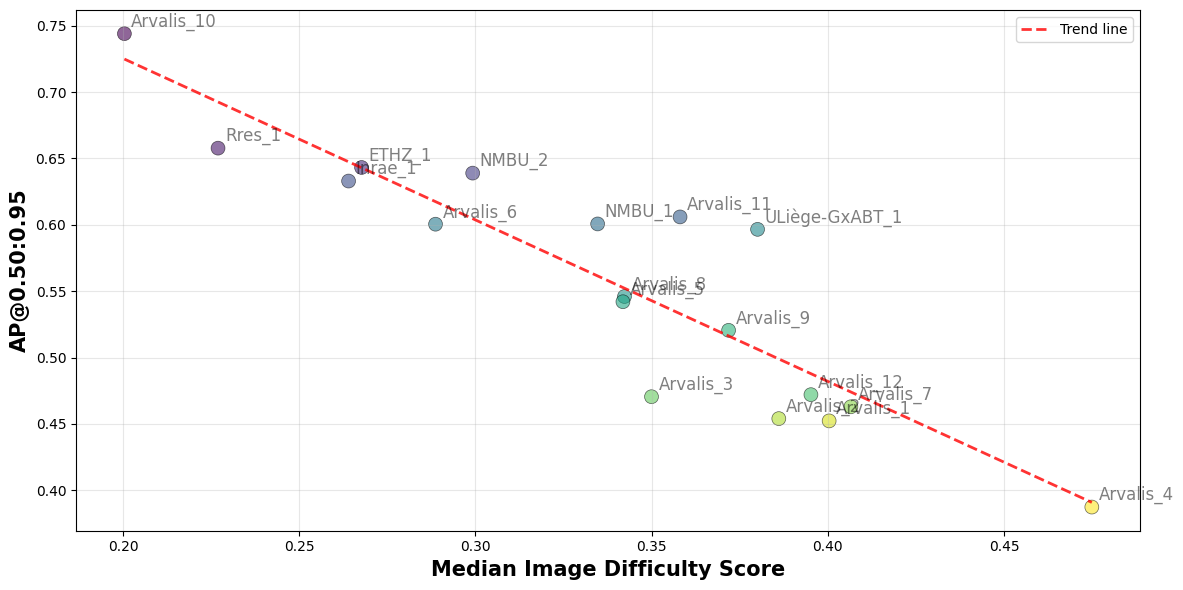
\includegraphics[width=\columnwidth]{gwhd_domain_score.png}
%   \caption{GWHD 2021: per-domain AP vs median image difficulty (MIS).}
%   \label{fig:gwhd_domain}
% \end{figure}

% \subsection{Copy-paste outcomes and failure analysis}
% \textbf{MinneApple: insufficient distribution shift under dense, sub-resolution conditions.}
% Across all four copy-paste conditions, AP changes are negligible and negative within seed variance (Table~\ref{tab:aug}).
% The critical control is \textbf{Score Low}: it increases the Medium fraction (31.5\%) relative to baseline (26.4\%),
% yet yields no AP improvement.
% This weakens ``suboptimal instance selection'' as the primary explanation and is more consistent with structural constraints:
% (i) a resolution ceiling dominated by Very Small objects (Table~\ref{tab:size_validation}),
% and (ii) a marginal density increase relative to the already-dense baseline (Obj/Img changes by ${\sim}1$--$2$),
% limiting the ability of copy-paste to introduce meaningfully new training signal.

% \textbf{GWHD 2021: domain-linked seed instability.}
% Score High augmentation yields near-zero mean gain but large seed sensitivity: across three seeds,
% performance ranges from a gain of $+0.042$ AP (seed 456) to a drop of $-0.055$ AP (seed 123).
% Given the strong domain difficulty--AP anticorrelation (Fig.~\ref{fig:gwhd_domain}), this variance is consistent with hard images concentrating in minority domains;
% score-guided sampling can therefore amplify domain imbalance, making outcomes sensitive to sampling order and initialization.

% \begin{table}[t]
% \centering
% \caption{MinneApple copy-paste results (3-seed mean). No condition yields a reliable gain.}
% \label{tab:aug}
% \footnotesize
% \setlength{\tabcolsep}{3.0pt}
% \renewcommand{\arraystretch}{0.95}
% \begin{tabular}{lccccc}
% \toprule
% \textbf{Condition} & \textbf{Obj/Img} & \textbf{V.\,Small} & \textbf{Small} & \textbf{Medium} & \textbf{AP$\pm\sigma$} \\
% \midrule
% Test set      & 37.11 & 17.2\% & 38.1\% & 44.7\% & --- \\
% \midrule
% Baseline      & 42.6  & 23.1\% & 50.5\% & 26.4\% & $0.353\pm0.005$ \\
% Random CP     & 44.0  & 23.5\% & 49.9\% & 26.5\% & $0.346\pm0.005$ \\
% Score High    & 43.9  & 26.5\% & 49.5\% & 23.9\% & $0.350\pm0.007$ \\
% Score Medium  & 43.2  & 22.6\% & 50.8\% & 26.6\% & $0.348\pm0.006$ \\
% Score Low     & 42.4  & 20.0\% & 48.5\% & 31.5\% & $0.348\pm0.003$ \\
% \bottomrule
% \end{tabular}
% \end{table}

% \subsection{Pre-augmentation diagnostic checklist}
% Across these benchmarks, MIS supports a practical triage from baseline outputs:
% (i) \textit{Information bottleneck}---hard objects concentrate in regimes with near-zero AP (e.g., sub-resolution sizes), implying limited usable capacity;
% (ii) \textit{Density-limited shift}---high baseline density implies that typical copy-paste ratios induce only marginal distribution shift even with ``correct'' sampling;
% (iii) \textit{Domain instability}---hard images cluster in minority domains (Fig.~\ref{fig:gwhd_domain}), so score-guided sampling can amplify imbalance and increase seed variance.

% % ----------------------------------------------------------
% \section{Conclusion}
% MIS reframes copy-paste augmentation from trial-and-error into a pre-augmentation diagnostic.
% On MinneApple and GWHD 2021, MIS aligns with size- and domain-level detection capacity and highlights failure modes consistent with dense, sub-resolution scenes and domain-driven instability.
% These findings are retrospective on two benchmarks under a fixed copy-paste protocol; prospective validation on datasets where copy-paste yields consistent gains remains necessary.
% When MIS indicates a resolution ceiling (near-zero AP in the dominant hard regime), duplicating pixels via copy-paste is unlikely to be sufficient.
% A plausible next direction is to evaluate augmentations that increase effective information content for hard cases (e.g., controlled super-resolution, domain-conditioned synthesis, or inpainting-based instance generation), while validating that generated samples remain in-distribution.

% {\footnotesize
% \begin{thebibliography}{00}
% \bibitem{kisantal2019augmentation}
% M.~Kisantal, Z.~Wojna, J.~Murawski, J.~Naruniec, and K.~Kyriakopoulos,
% ``Augmentation for small object detection,''
% in \textit{Proc. Int. Conf. Adv. Comput., Commun. Informat.\ (ICACCI)}, 2019, pp.~193--197.

% \bibitem{ghiasi2021simple}
% G.~Ghiasi \textit{et~al.},
% ``Simple copy-paste is a strong data augmentation method for instance segmentation,''
% in \textit{Proc. IEEE/CVF CVPR}, 2021, pp.~2918--2928.

% \bibitem{hani2020minneapple}
% N.~Hani, P.~Roy, and B.~Bhanu,
% ``MinneApple: A benchmark dataset for apple detection and segmentation,''
% \textit{IEEE Robot.\ Autom.\ Lett.}, vol.~5, no.~2, pp.~852--858, 2020.

% \bibitem{david2021global}
% E.~David \textit{et~al.},
% ``Global Wheat Head Detection (GWHD) dataset,''
% \textit{Plant Phenomics}, 2021.
% \end{thebibliography}
% }

% \end{document}